\section{Unweighted API Importance}
\label{sec:syspop:security}

\Usagemetric{} is weighted by the number of installations
of applications that use the API.
As a result, one ubiquitous application can cause the \usagemetric{} of an API it uses to be close to 100\%.
This section observes trends for APIs with multiple variants, using an additional 
\unwusagemetric{} metric. 
We remove the weighting by installation frequency to focus on 
trends in developer behavior.


%In addition to migrating applications to easier-to-secure APIs, 
%%an \unwusagemetric{} provides insights about developers' preferences about using different variants of 

Once an API has been identified as having a security risk, and a more secure variant
is developed, one might wish to know how many 
%But, this misses the other side of the puzzle.
%While security researchers are interested in
vulnerable packages are still in the wild,
and how many have moved to less exploit-prone APIs.
%In particular, one is concerned with adoption of API variants that are less prone to error or exploit.
%and deprecation of problematic APIs.
Similarly, one might want to know how many applications have not migrated away from a deprecated API,
even if these applications are not widely used.

\vspace{0.1in}
{\noindent
\fbox{\begin{minipage}{\linewidth}
\setlength{\parindent}{-0.1in}
\setlength{\leftskip}{0.1in}
\setlength{\rightskip}{0.1in}
Definition: {\bf \Unwusagemetric{}.} \\
For a given API, the probability an application (package) uses that API, irrespective
of probability of installation.
\end{minipage}}}
\vspace{0.1in}

%\begin{figure}[t]
%\vspace{-0.2in}
%\center{
%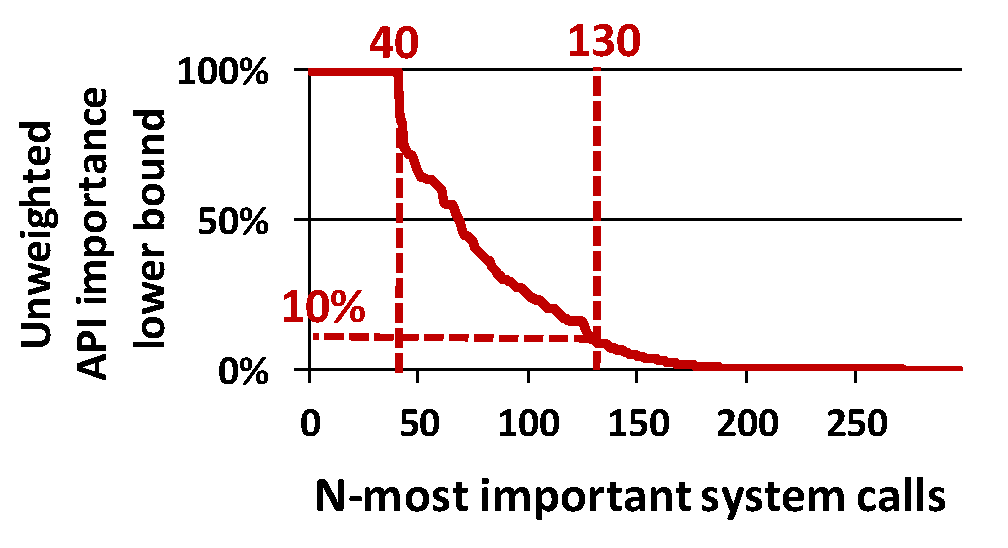
\includegraphics[width=3.6in]{syspop/figures/unweighted-syscall-popularity-all.pdf}
%}
%\footnotesize
%\caption[\Unwusagemetric{} of Linux system calls]
%{The trend of \unwusagemetric{} in N-most important system calls among total \syscallnum{} system calls of \osversion{} with Linux kernel \kernelversion{}.}
%\label{fig:unweighted-syscall-popularity-trend}
%\end{figure}

%We begin by looking at the \unwusagemetric{} of each system call. Figure~\ref{fig:unweighted-syscall-popularity-trend} shows the 
%distribution of system calls across packages. 
%Recall that using \usagemetric{},
%over two-thirds of system calls on Linux are required by 
%at least one application on every installation.
%Using \unwusagemetric{},
%Figure~\ref{fig:unweighted-syscall-popularity-trend} suggests that only 40 system calls are used by all packages,
%and 130 system calls
%are used by at least 10\% of packages.
%%In terms of a prototype maximizing its coverage of potential applications with no concern for overall usability, 130 system calls is the optimal 
%%balance of effort and reward.
%Over half of Linux system calls are used by less than 10\% of packages.  

%%% Thus, changing the security guarantees for just 130 system calls can ensure that 90\% of the packages
%%% are secured. However, we should keep in mind that this does not mean 90\% of the systems are secured as there may be some API used by 
%%% an ubiquitous package that is not secured.

One family of APIs prone to security problems are the %with security issues   that have been considered problematic
{\tt set*id} API family.
%The fundamental problem is that
Many of the {\tt set*id} APIs
have subtle semantic differences across different Unix variants.
%~\citep{chen02setuid}.
Chen et al.~\citep{chen02setuid} conclude that 
{\tt setresuid} has the clearest semantics 
across all Unix flavors. 
%BSD, System V and Linux have different interpretation of 
%other uid-setting system calls such as setuid, setreuid and seteuid. 
Table~\ref{tab:syspop:secure-api} shows the \unwusagemetric{} 
of {\tt set*id} and {\tt get*id} system calls.
Most packages have 
adopted the more clear and secure interface. 
System calls {\tt setuid}, {\tt setreuid}, and {\tt setresuid} have
\unwusagemetric{} of 15.67\%, 1.88\% and 99.68\% respectively. 
%However, some packages
%are still using the older interfaces, and package maintainers or distribution security teams
%may want to push patches to these lingering instances more aggressively.
%The \unwusagemetric{} trend of {\tt set*gid} is similar to
%that of {\tt set*uid}.
However, for {\tt get*id} system calls, the \unwusagemetric{} suggests that the {\tt getres*id}
system calls %with the clearest semantics are not preferred.
are only used by roughly 36\% of packages.
%Package maintainers or distribution security teams
%may want to rectify this case.

Directory operations have a long history of exploitable race conditions~\citep{tocttou-truck, wei05fast, races-usenix05}, or time-of-check-to-time-of-use (TOCTTOU) vulnerabilities.
%Another security concern that exists in file system calls that operate on dire
%is {\em atomicity}.
In a privileged application, one system call (e.g., {\tt access}) checks 
the user's permission, and a second call operates on the file.
%This system call is primarily used
%by privileged applications, such as setuid-to-root binaries.
%The {\tt access} call is used to avoid potential ``confused deputy'' problems~\citep{Hardy:1988:CD:54289.871709},
%by determining the invoking user's authority
%by checking the access rights of the calling process's real UID and GID
%instead of the effective ID.
%The problem is that {\tt access}
%are vulnerable to 
%time-of-check-to-time-of-use (TOCTTOU) attacks~\citep{tocttou-truck}.
%The attacker can change the resource's state 
%between the check and the use in such a way that it invalidates the results of the check.
There are countermeasures that effectively walk the directory
hierarchy in user space~\citep{tsafrir08tr}.
This approach replaces calls like {\tt access} with {\tt faccessat},
and similar variants.
%The atomic version of these system calls, such as
%{\tt faccessat}, avoids this attack by interpreting the path relative to
%an already open file descriptor~\citep{tsafrir08tr}.
Table~\ref{tab:syspop:secure-api} shows the current \unwusagemetric{} of
{\tt *at} system call variants and their older counterparts.
We observed that the \unwusagemetric{} of
the race-prone {\tt access} is still high (74.24\%), whereas {\tt faccessat} is only 0.63\%.
This suggests about 75\% of the
packages use the more vulnerable {\tt access} system call instead of the more secure one.
%This indicates that perhaps more outreach is needed on this issue.
%Similar to {\tt access} and {\tt faccessat}, a few more system calls designed to prevent TOCTTOU attacks
%are shown in
%more of this types of system call variants.
%The \unwusagemetric{} trend for the other system calls is similar, except for
%{\tt fstat} and {\tt newfstatat} which are both ubiquitously used.

\begin{table}[t!b!]
\footnotesize
\centering
\begin{tabular}{m{1.2in}>{\raggedleft\arraybackslash}m{1.2in}m{1.2in}>{\raggedleft\arraybackslash}m{1.2in}}
\toprule
{\bf Insecure API} & {\bf \UnwusageMetric{}} & {\bf Secure API} & {\bf \Unwusagemetric{}}\\
\midrule
\multicolumn{4}{c}{\bf Unclear vs. Well-defined ID Management Semantics} \\
\midrule
\addlinespace
{\tt setuid}   & 15.67\% & \multirow{2}{*}{\tt setresuid} & \multirow{2}{*}{99.68\%} \\
{\tt setreuid} &  1.88\% & & \\
\addlinespace {\tt setgid}   & 12.07\% & \multirow{2}{*}{\tt setresgid} & \multirow{2}{*}{99.68\%} \\
{\tt setregid} &  1.24\% & & \\
\addlinespace
{\tt getuid}   & 99.81\% & \multirow{2}{*}{\tt getresuid} & \multirow{2}{*}{36.19\%} \\
{\tt geteuid}  & 55.15\% & & \\
\addlinespace
{\tt getgid}   & 99.81\% & \multirow{2}{*}{\tt getresgid} & \multirow{2}{*}{36.14\%} \\
{\tt getegid}  & 48.87\% & & \\
\addlinespace
\midrule
\multicolumn{4}{c}{\bf Nonatomic vs. Atomic Directory operations} \\
\midrule
{\tt access}   & 74.24\% & {\tt faccessat}  & 0.63\% \\
\addlinespace
{\tt mkdir}    & 52.07\% & {\tt mkdirat}    & 0.34\% \\
%\addlinespace
%& {\tt mknod}    &  5.86\% & {\tt mknodat}    & 0.26\% \\
%\addlinespace
{\tt rename}   & 43.18\% & {\tt renameat}   & 0.30\% \\
%\addlinespace
%& {\tt symlink}  & 21.93\% & {\tt symlinkat}  & 0.34\% \\
%\addlinespace
{\tt readlink} & 46.38\% & {\tt readlinkat} & 0.50\% \\
\addlinespace
%& {\tt link}     & 28.04\% & {\tt linkat}     & 0.28\% \\
%\addlinespace
%& {\tt utimes}   & 17.90\% & {\tt futimesat}  & 0.20\% \\
%\addlinespace
%& {\tt chown}    & 24.59\% & \multirow{2}{*}{\tt fchownat}   & \multirow{2}{*}{ 0.23\%} \\
%& {\tt fchown}   & 27.14\% & & \\
{\tt chown}    & 24.59\% & {\tt fchownat}   & 0.23\% \\
{\tt chmod}    & 39.80\% & {\tt fchmodat}   & 0.13\% \\
%& {\tt stat}     & 99.80\% & \multirow{2}{*}{\tt newfstatat} & \multirow{2}{*}{99.79\%} \\
%& {\tt fstat}    & 99.80\% & & \\ {\tt stat}     & 99.80\% & {\tt newfstatat}   & 99.79\% \\
%& {\tt chmod}    & 39.80\% & \multirow{2}{*}{\tt fchmodat}   & \multirow{2}{*}{ 0.13\%} \\
%& {\tt fchmod}   & 32.78\% & & \\
\bottomrule
\end{tabular}
\caption[\Unwusagemetric{} of secure and insecure API variations]
{\Unwusagemetric{} of secure and insecure API variations. Higher is more important.}
\label{tab:syspop:secure-api}
\end{table}


In addition to security-related hints, \unwusagemetric{}
indicates whether obsolete APIs have been replaced by newer variants.
%\fixmedp{Skimming the waitit manual, it is not obvious that wait4 is actually obsolete;
%in fact, I think it is system-specific and more precise (similar to dup3 below).}
For instance, {\tt wait4} system call is considered obsolete~\citep{wait4man},
and the alternative {\tt waitid} is preferred, as it more precisely specifies which child state changes to wait for. %\fixmetsai{kernel version? cite?}\fixmedp{why?}
However, \unwusagemetric{} of {\tt wait4} and {\tt waitid} is 60.56\% and 0.24\%, respectively.
This indicates that 60\% of the packages are still using the older {\tt wait4} system call.
%This is another area of concern that needs to be notified to the maintainers of these packages.
Table~\ref{tab:syspop:new-api} shows similar trend for some other system calls.
Our dataset provides more opportunity for system developers
to actively communicate with application developers,
in order to speed up the process of retiring problematic APIs. 

%\callout{Adoption of newer, preferred API variants is often slow, and 
%kernel developers could benefit from an easy mechanism to identify
%relevant developers.}

Some APIs are specific to a particular OS,
such as Linux,
and often have more portable variants.
Table~\ref{tab:syspop:linux-specific} shows the comparison between
Linux-specific APIs and their generic variants.
The results show most developers prefer portable or generic APIs
more than Linux-specific APIs.
Except {\tt pipe2}, most API variants that are Linux-specific
have \unwusagemetric{} lower than 10 percent.
\fixmedp{Can you comment on why pipe2 is popular?}
%Moreover, \unwusagemetric{} also gives us insights about developer preference over multiple versions of similar API. For example, whenever possible,
%developers choose the API to maximize the portability of the application. As a result, the \unwusagemetric{} of Linux specific version of system call API is very low compared to their generic counterparts as shown in table ~\ref{tab:linux-specific}.

Finally, we consider system calls with multiple variants
where one version has increased functionality.
%neither is any of them more secure than their siblings.
%Some of them are just alternative to each other,
%or one is simply a more powerful version (more functionality;
%accepting more arguments) of the other.
%The existence of these API variants is caused by arbitrary choices
%made by the OS developers.
%In addition to some system call variants being Linux specific, in some cases, that is not the factor for developer preference of one API variant over the other.
Table~\ref{tab:syspop:prefer-api} shows the difference %of \unwusagemetric{}
between these system calls.
%which are either alternative to each other,
%or one is simply a more powerful version (more functionality; accepting more arguments) of the other.
%In a few cases, like {\tt recvfrom} or {\tt sendto},
%a significant fraction of the developers choose
%the more powerful version of the system calls ({\tt recvmsg} or {\tt sendmsg})
%or more functionality. 
Interestingly, more developers chose the less powerful variants,
such as using {\tt select} over {\tt pselect6}, or {\tt dup2} over {\tt dup3}.
This indicates that more often than not, developers choose simplicity 
unless a task demands the functionality of a more powerful API variant.

\begin{table}[t!b!]
\footnotesize
\centering
\begin{tabular}{m{1.2in}>{\raggedleft\arraybackslash}m{1.2in}m{1.2in}>{\raggedleft\arraybackslash}m{1.2in}}
\toprule
{\bf Old API} & {\bf \UnwusageMetric{}} & {\bf New API} & {\bf \UnwusageMetric{}}\\
\midrule
{\tt getdents} & 99.80\% & {\tt getdents64} & 0.08\% \\
\addlinespace
{\tt utime} & 8.57\% & {\tt utimes} & 17.90\% \\
\addlinespace
{\tt fork} & 0.07\% & \multirow{2}{*}{\tt clone} & \multirow{2}{*}{99.86\%} \\ 
{\tt vfork} & 99.68\% & & \\
\addlinespace
{\tt tkill} & 0.51\% & {\tt tgkill} & 99.80\% \\
\addlinespace
{\tt wait4} & 60.56\% & {\tt waitid} & 0.24\% \\
\bottomrule
\end{tabular}%
\caption[\Unwusagemetric{} of old and new API variations.]
{\Unwusagemetric{} of old (generally deprecated) and new (preferred) API variations. Higher is more important.}
\label{tab:syspop:new-api}
\end{table}%


\begin{table}[t!b!]
\footnotesize
\centering
\begin{tabular}{m{1.2in}>{\raggedleft\arraybackslash}m{1.2in}m{1.2in}>{\raggedleft\arraybackslash}m{1.2in}}
\toprule
{\bf Linux Specific API} & {\bf \Unwusagemetric{}} & {\bf Portable / Generic API} & {\bf \Unwusagemetric{}}\\
\midrule
{\tt preadv} & 0.15\% & {\tt readv} & 62.23\% \\
%\addlinespace
{\tt pwritev} & 0.16\% & {\tt writev} & 99.80\% \\
\addlinespace
{\tt accept4} & 0.93\% & {\tt accept} & 29.35\% \\
\addlinespace
{\tt ppoll} & 3.90\% & {\tt poll} & 71.07\% \\
\addlinespace
{\tt recvmmsg} & 0.11\% & {\tt recvmsg} & 68.82\% \\
%\addlinespace
{\tt sendmmsg} & 5.17\% & {\tt sendmsg} & 42.49\% \\
\addlinespace
{\tt pipe2} & 40.33\% & {\tt pipe} & 50.33\% \\
\bottomrule
\end{tabular}%
\caption[\Unwusagemetric{} of other API variants]
{\Unwusagemetric{} of other API variants,
and comparison between Linux-specific versions and more portable or generic versions. Higher is more important.}
\label{tab:syspop:linux-specific}%
\end{table}%


\begin{table}[t!b!]
\footnotesize
\centering
\begin{tabular}{m{1.2in}>{\raggedleft\arraybackslash}m{1.2in}m{1.2in}>{\raggedleft\arraybackslash}m{1.2in}}
\toprule
{\bf Linux API} & {\bf \Unwusagemetric{}} & {\bf Alternative API} & {\bf \Unwusagemetric{}}\\
\midrule
{\tt read} & 99.88\% & {\tt pread64} & 27.23\% \\
{\tt select} & 61.53\% & {\tt pselect6} & 4.13\% \\
\addlinespace
\multirow{2}{*}{\tt dup3} & \multirow{2}{*}{8.72\%} & {\tt dup2} & 99.75\% \\
& & {\tt dup} & 66.64\% \\
\addlinespace
{\tt recvmsg} & 68.82\% & {\tt recvfrom} & 53.80\% \\
{\tt sendmsg} & 42.49\% & {\tt sendto} & 71.71\% \\
%\addlinespace
%{\tt chdir} & 44.61\% & {\tt fchdir} & 2.20\% \\
\bottomrule
\end{tabular}%
\caption[\Unwusagemetric{} among similar API variants]
{\Unwusagemetric{} among similar API variants. Higher is more important.}
\label{tab:syspop:prefer-api}%
\end{table}%

 
%\callout{Developers  prefer the most portable or the simplest API option among variations of same system call.}
